\section{What is Java?}

\subsection{Java}

\begin{frame}{Brief Overview}

\begin{itemize}
\item Java is a \emph{programming language}. \pause
\item One of the most popular programming languages today (July 7\textsuperscript{th}, 2014) \pause
\item Developers use Java to make programs for operating systems such as Windows, iOS, Linux, and Android. \pause
\item Has a ``write once run anywhere" philosophy, and uses a virtual machine. \pause
\item More importantly it has been used for a few notable games...

\end{itemize}

\end{frame}

\begin{frame} Game \# 1
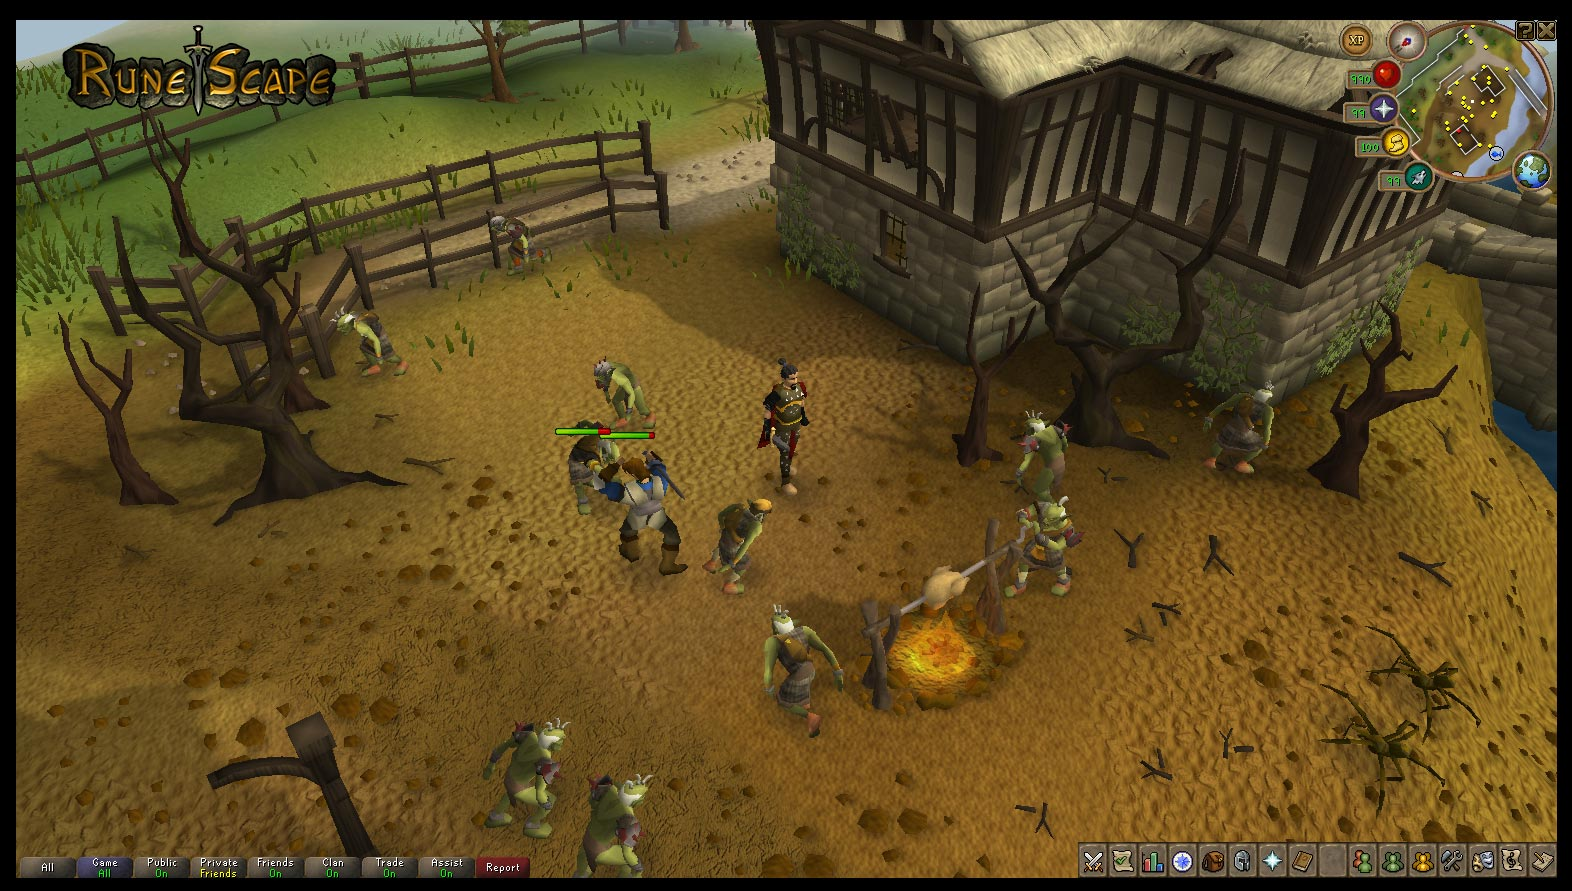
\includegraphics[width = 10cm]{runescape}

\end{frame}

\begin{frame} Game \# 2
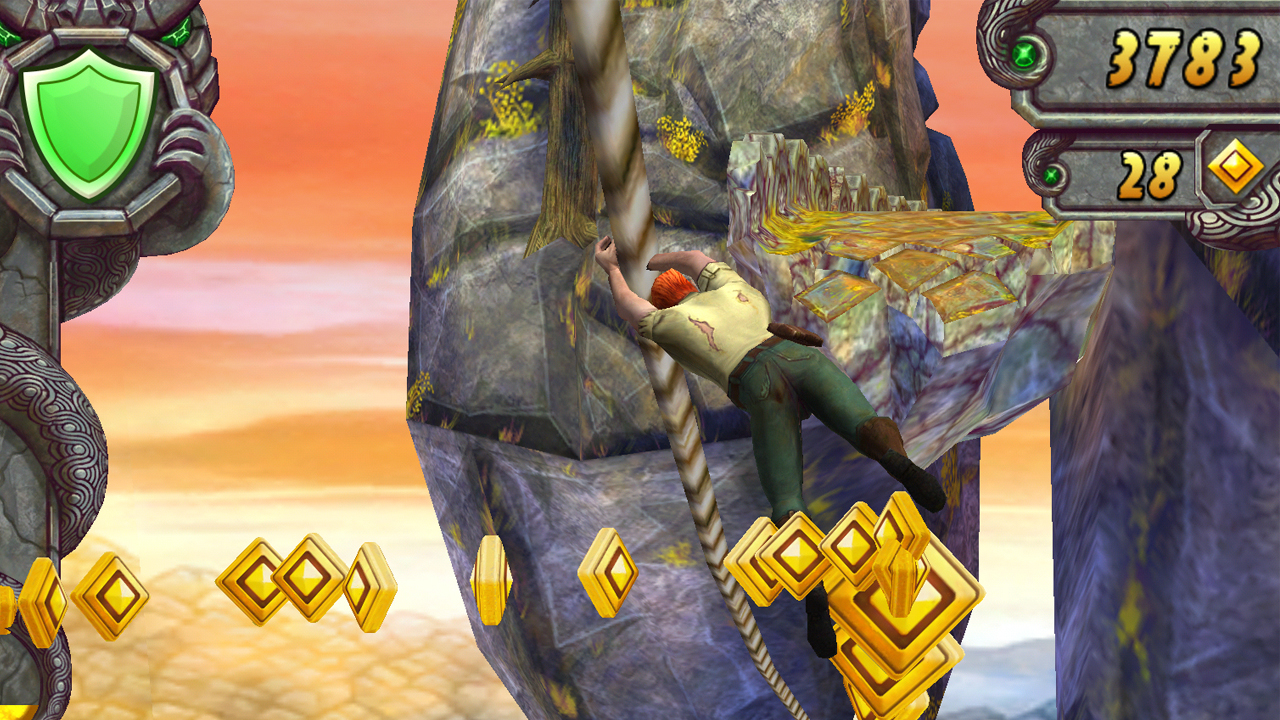
\includegraphics[width = 10cm]{templerun}

\end{frame}

\begin{frame} Game \# 3
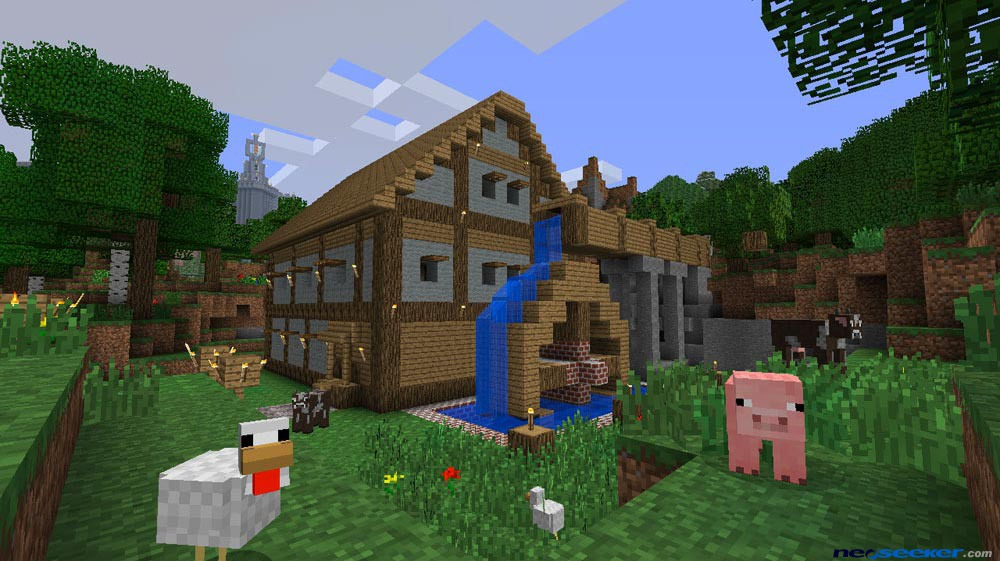
\includegraphics[width = 10cm]{minecraft}

\end{frame}



\begin{frame}{Why Java?}
\begin{itemize}
\item There are several careers for Java programmers due to the language's popularity.\pause
\item It is a necessary language for Android development. \pause
\item It is object oriented. \pause
\item It has extensive libraries and good community support. \pause
\end{itemize}
\emph{However, is Java (or any other language) the best? Certain languages perform better at certain tasks. More importantly, it is easy to learn other programming languages once you know one.}
\end{frame}

\begin{frame}{Deep Questions}
\begin{itemize}
\item What is a program?\\ \pause

\emph{A program is a set of instructions that when read by a computer perform a certain task. By a set of instructions, we mean the binary sequences that a CPU can read.} \pause

\item How are programs made?\\ \pause
\emph{They are compiled: Idea $\Rightarrow$ source code $\Rightarrow$ (Java bytecode $\Rightarrow$) program.}
\pause

\item How do games work?\\ \pause
\emph{Games are some of the most interesting programs out there. Games have to perform several intense calculations several times per second, requiring very cunning algorithms.}
\end{itemize}
\end{frame}

\begin{frame}{What will we do in this class?}
\begin{itemize}
\item ALOT!!!! \pause
\item First, we will learn the basics of programming:
    \begin{itemize}
    \item How to save, compile, and run your code. \pause
    \item Syntax: \texttt{;, =, "", int}... \pause
    \item Lots of loops, and some data structures \pause
    \item Libraries: util.Scanner, swing.JFrame, util.Date, io.File...
    \end{itemize}
\end{itemize}

\end{frame}

\begin{frame}{What else will we do in this class?}
\begin{itemize}
\item Algorithms:
    \begin{itemize}
    \item Methods \pause
    \item Recursion \pause
    \end{itemize}
\item GUIs and graphics! \pause
\item Use Eclipse IDE \pause
\item Make an RPG (or other game perhaps?)
\end{itemize}
\end{frame}


\subsection{Games}

\begin{frame}{What will our games look like?}
\begin{center}
Our games will not look like this:\\
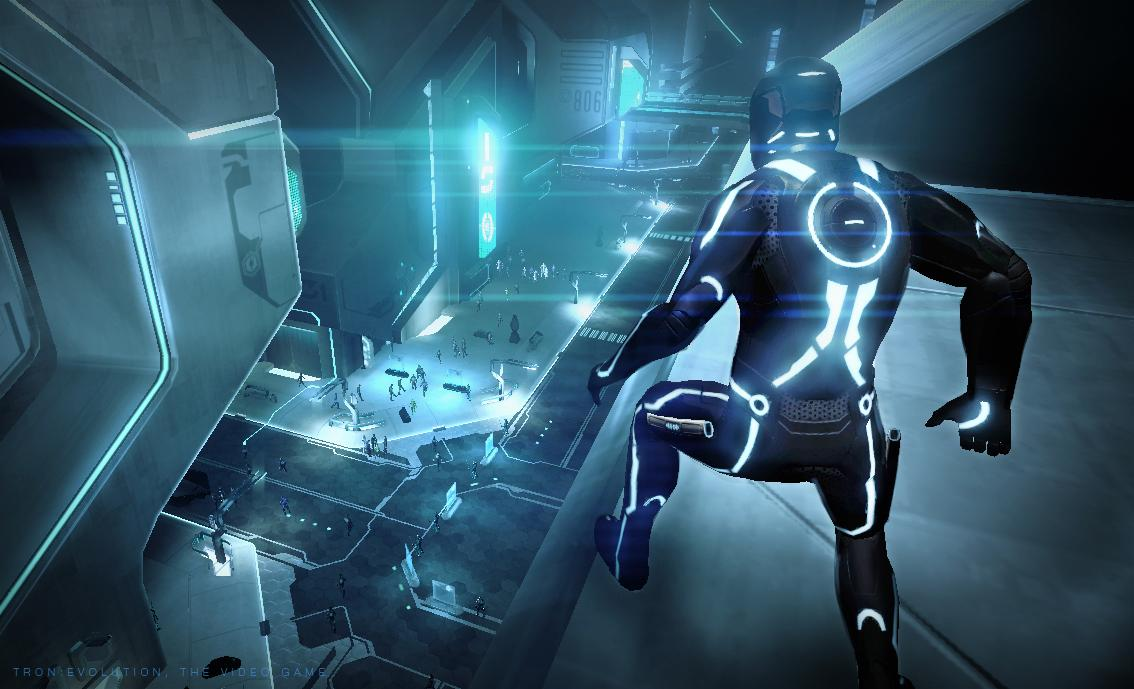
\includegraphics[width = 7cm]{hightech}\\ \pause
\emph{but that's ok.}
\end{center}

\end{frame}

\begin{frame}{Progression}
\begin{center}
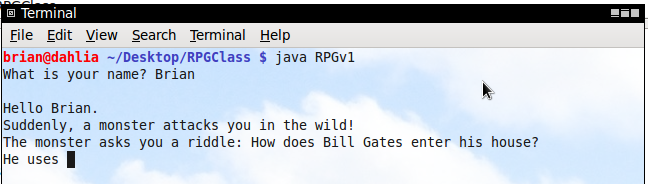
\includegraphics[width = 7cm]{game1} \\ \pause
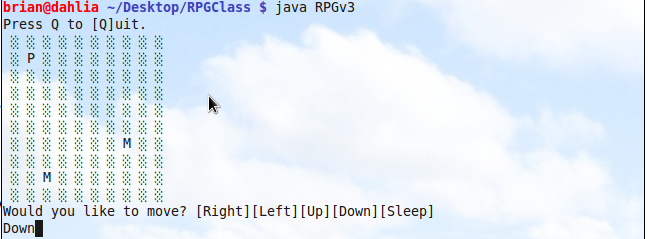
\includegraphics[width = 7cm]{game2} \\ \pause
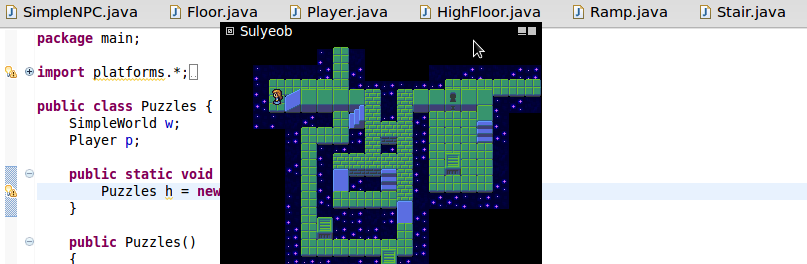
\includegraphics[width = 7cm]{game3} \\ \pause


\end{center}
\end{frame}

\begin{frame}{Historical Similarity}
\begin{center}
In a way, we will be tracing the history of game development:
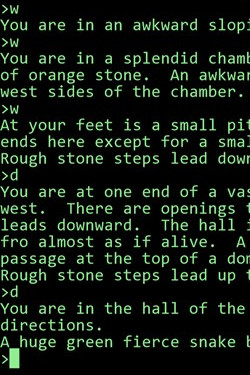
\includegraphics[width = 3cm, valign = c]{colossalcaveadventureS} $\Rightarrow$
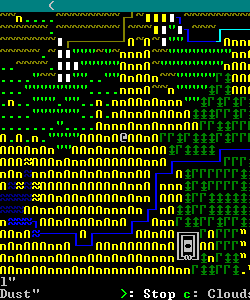
\includegraphics[width = 3cm, valign = c]{dwarffortressS} $\Rightarrow$
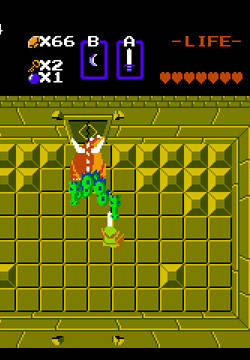
\includegraphics[width = 3cm, valign = c]{zeldaS} \\
\end{center}
\end{frame}

\begin{frame}{What's the difference between 2d and 3d?}
\begin{center}
Mostly how the graphics are rendered.\\
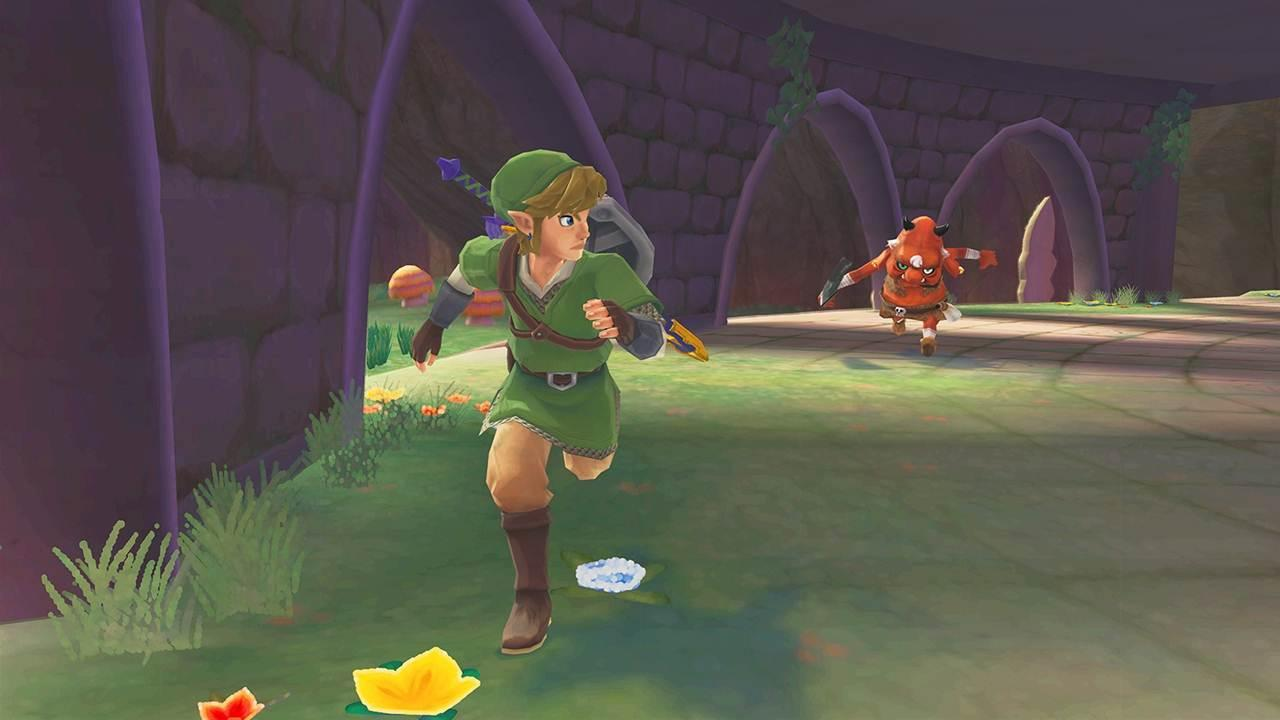
\includegraphics[width = 11cm]{3dzelda}
\end{center}
\end{frame}

\section{Let's Begin!}
\subsection{Hello World!}
\begin{frame}{Your first program}
\begin{itemize}
\item Login:
\begin{itemize}
\item Username: osummer
\item Password: y1ycwd8y
\end{itemize} \pause
\item Open Notepad (\code{\texttt{All Programs > Accessories > Notepad}})\pause
\item Save your blank file as Hello.java on your flash drive.\pause
\end{itemize}
\end{frame}

\begin{frame}[fragile]{The Code}
\begin{itemize}
\item Type in the following \emph{exactly} as it is shown:\\
\begin{semiverbatim}\code{
public class Hello\{
    public static void main(String[] args)\{
        System.out.println("Hello World!");
    \}
\}
}
\end{semiverbatim}
\item Save.
\item Open the Command Prompt (\code{\texttt{All Programs > Accessories > Command Prompt}}).

\end{itemize}
\end{frame}

\begin{frame}[fragile]{The Command Prompt}
\begin{itemize}
\item Find your flash drive (\code{\texttt{Computer > F:\textbackslash, G:\textbackslash, H:\textbackslash, etc.}})\pause
\item Once you find the name of your drive type it into the Command Prompt and press Enter:
\begin{semiverbatim}\code{
C:{\textbackslash}Users{\textbackslash}Admin> G:

G:{\textbackslash}>
}\end{semiverbatim}
\item To see the files in a directory type \code{\texttt{dir}}.
\item To move between directories type \code{\texttt{cd <directory\_name>}}.
\end{itemize}
\end{frame}


\begin{frame}[fragile]{The Command Prompt}
\begin{itemize}
\item To compile your code use \code{\texttt{javac <name\_of\_class>.java}}.
\begin{semiverbatim}\code{
G:{\textbackslash}RPGClass\textbackslash> javac Hello.java

G:{\textbackslash}RPGClass\textbackslash>
}\end{semiverbatim} \pause
\item Then run your code using \code{\texttt{java <name\_of\_class>}}.
\begin{semiverbatim}\code{
G:{\textbackslash}RPGClass\textbackslash> java Hello
Hello World!

G:{\textbackslash}RPGClass\textbackslash>
}\end{semiverbatim}
\item Congratulations! You have completed your first program.
\end{itemize}
\end{frame}

\begin{frame}[fragile]{How does the code work?}

\begin{semiverbatim}\code{
\addcorners{1}{public} \addcorners{2}{class} \addcorners{3}{Hello}\{
    \addcorners{4}{public static void main(String[] args)}\{
        \addcorners{5}{System.out.println("Hello World!")};
    \}
\}
}\end{semiverbatim}
\only<1>{\begin{tikzpicture}[overlay, remember picture]
            % Define the circle paths
            \draw [white,ultra thick,rounded corners](1.north west) -- (1.north east) --
            (1.south east) -- (1.south west) -- cycle;

            \end{tikzpicture}}

\only<2>{\begin{tikzpicture}[overlay, remember picture]
\draw [red,ultra thick,rounded corners](2.north west) -- (2.north east) --
            (2.south east) -- (2.south west) -- cycle;
\end{tikzpicture}}


\only<3>{\begin{tikzpicture}[overlay, remember picture]
\draw [red,ultra thick,rounded corners](3.north west) -- (3.north east) --
            (3.south east) -- (3.south west) -- cycle;
\end{tikzpicture}}


\only<4>{\begin{tikzpicture}[overlay, remember picture]
\draw [red,ultra thick,rounded corners](4.north west) -- (4.north east) --
            (4.south east) -- (4.south west) -- cycle;
\end{tikzpicture}}


\only<5>{\begin{tikzpicture}[overlay, remember picture]
\draw [red,ultra thick,rounded corners](5.north west) -- (5.north east) --
            (5.south east) -- (5.south west) -- cycle;
\end{tikzpicture}}


\only<1>{Modifier: \emph{public} means that this class can be seen by all other classes.}
\only<2>{Class: all java programs are written within classes. This keyword tells java that what follows is the name of a class}
\only<3>{Hello: the name of the class. Since this class is public, the class name, and the file name must be the same. (Hello.java)}
\only<4>{public static void main(String[] args): This is a \emph{method} with an \emph{argument}. When ever the program is run, this method is called.}
\only<5>{System.out.println(): this method prints a \emph{String} to the terminal.}
\only<6>{\texttt{"Hello World!"}: this is a string.}

\end{frame}


\begin{frame}[fragile]{What are we doing in the Command Prompt?}
\begin{semiverbatim}\code{
G:{\textbackslash}RPGClass\textbackslash> javac Hello.java

G:{\textbackslash}RPGClass\textbackslash>
}\end{semiverbatim}
\begin{center}
This compiles the Java code (written using human readable characters) into Java bytecode.
\end{center}

\pause
\begin{semiverbatim}\code{
G:{\textbackslash}RPGClass\textbackslash> java Hello
Hello World!

G:{\textbackslash}RPGClass\textbackslash>
}\end{semiverbatim}
\begin{center}
This runs the Java bytecode, by using a JIT compiler. The JIT compiler translates the Java bytecode into the bytecode used by your computer.
\end{center}
\end{frame}

\subsection{Hello World Extended!}
\begin{frame}{What is a String?}
\begin{itemize}
\item Before we upgrade our program, let's learn about variables.
\item A string is a sequence of characters surrounded by quotes (\code{\texttt{""}}). \pause
\item Which of the following are Strings?
\begin{itemize}
\item \code{\texttt{"Hello World!"}} \pause \emph{Yes}
\item \code{\texttt{"12,350"}} \pause \emph{Yes}
\item \code{\texttt{How are you doing today?}} \pause \emph{No}
\item \code{\texttt{'Hi, my name is Brian!'}} \pause \emph{No}
\item \code{\texttt{"OMG, I learned sooo much in the coding class today.""}} \pause \emph{No}
\item \code{\texttt{"Then the instructor asked, \textbackslash"Are these strings?\textbackslash"."}} \pause \emph{Yes}
\end{itemize}

\end{itemize}
\end{frame}

\begin{frame}[fragile]{What is a variable?}
\begin{itemize}
\item Variables associate a value with a type and a name.\pause
\item The type of a variable tells the compiler what kind of variable we have. \pause
\item The name of a variable is a \emph{unique} identifier. \pause
\item We can declare a variable by typing a type and a name:
\begin{center}
\begin{semiverbatim}\code{String message;}\end{semiverbatim}
\end{center}
\item Notice the ``;" at the end. A ; signifies the end of a \emph{statement}.
\item We can also assign a value to a variable:
\begin{center}
\begin{semiverbatim}\code{message = "Hello World!";}\end{semiverbatim}
\end{center}
\end{itemize}
\end{frame}

\begin{frame}{Pop Quiz!}
\begin{center}
Does Hello.java contain any statements?
\end{center}
\end{frame}


\begin{frame}[fragile]{Continuing on...}
\begin{itemize}
\item We can also declare and assign a variable in the same statement:
\begin{center}
\begin{semiverbatim}\code{String message = "Hello World!";}\end{semiverbatim}
\end{center} \pause
\item Edit Hello.java to print a message from a stored variable.
\begin{semiverbatim}\code{String <name> = "<your text here>";
System.out.println(<name>);
}\end{semiverbatim}
\item Try to declare another variable that has the same name as your variable. What happens when you try to compile?
\item Print your string once, then reassign a different value to it (Create a different message). Print again. What happens?
\end{itemize}
\end{frame}


\begin{frame}[fragile]{Getting arguments from the Command Prompt.}

\begin{itemize}
\item Remember \texttt{String[] args}? We can pass a value into the \emph{array} args when running our code.
\item Try the following code:
\end{itemize}
\begin{semiverbatim}\code{
public class HelloExtended\{
    public static void main(String[] args)\{
        System.out.println("Hello "+args[0]+"!");
    \}
\}
}\end{semiverbatim}
\end{frame}

\begin{frame}[fragile]{Running with Arguments.}
\begin{itemize}
\item When running the code try entering in different words:
\begin{semiverbatim}\code{
G:{\textbackslash}RPGClass\textbackslash> java Hello Brian
Hello Brian!

G:{\textbackslash}RPGClass\textbackslash>
}\end{semiverbatim}
\item Try to enter in more than one word. What happens?
\end{itemize}
\end{frame}

\begin{frame}{Other kinds of variables}
\begin{itemize}
\item int: positive or negative whole numbers. Ex:
\begin{itemize}
\item 1
\item 25632
\item -50
\item 0
\end{itemize}\pause
\item double: numbers that contain a decimal:
\begin{itemize}
\item 1.0
\item 5.5
\item -4672.3356
\item -0.00000001
\end{itemize}
\end{itemize}

\end{frame}


\begin{frame}{Other kinds of variables}
\begin{itemize}
\item char: a single char, surrounded by \code{\texttt{''}}. Ex:
\begin{itemize}
\item \texttt{'a'}
\item \texttt{'b'}
\item \texttt{'4'}
\item \texttt{'\$'}
\end{itemize} \pause
\item boolean: contains either \emph{true} or \emph{false}
\begin{itemize}
\item true
\item false
\end{itemize}
\end{itemize}
\end{frame}

\begin{frame}[fragile]{Some Operators}
\begin{semiverbatim}\code{
int x = 3 + 2; \pause
x = x - 5; \pause
x += 4; \pause
x = x * 3; \pause
int y = x / 5; \pause
x = x \% 5; \pause
x++; \pause
int z = -y; \pause
double w = 12.0;
w /= 5; \pause
String s = "I am " + 14 + 'y' + 'e' + "ars";
}\end{semiverbatim}
\end{frame}


\begin{frame}{Pre-Lunch Exercise}
\begin{center}
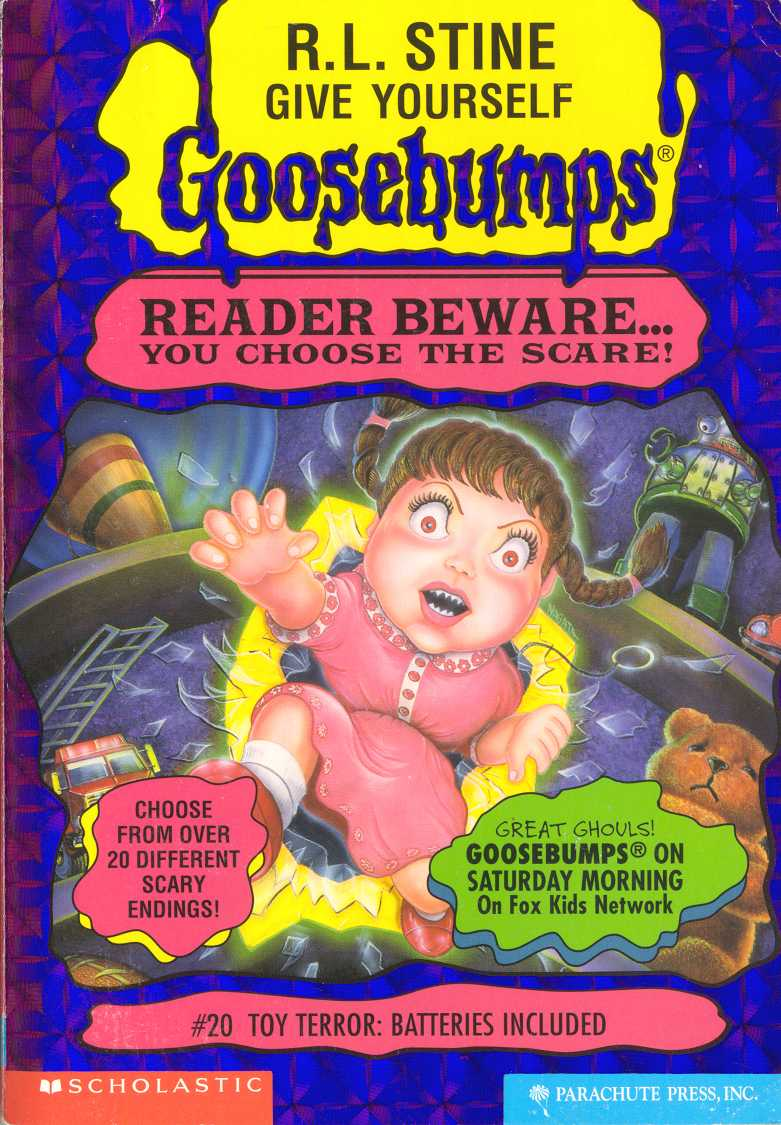
\includegraphics[width = 4.5cm]{goosebumps}
\end{center}
\end{frame}
